\documentclass[border=3pt]{standalone}
% Shared preamble for standalone TikZ figures (colors match the slide theme).
\usepackage[T1]{fontenc}
\IfFileExists{sourcesanspro.sty}{\usepackage[default]{sourcesanspro}}{\usepackage[scaled=0.92]{helvet}\renewcommand{\familydefault}{\sfdefault}}
\usepackage{xcolor,tikz}
\usetikzlibrary{arrows.meta,positioning,calc,shapes.geometric,decorations.pathmorphing,decorations.pathreplacing,backgrounds,fit}
\definecolor{fsNavy}{HTML}{1B365D}
\definecolor{fsAccent}{HTML}{C8102E}
\definecolor{fsGold}{HTML}{D39B1E}
\definecolor{fsTeal}{HTML}{1F7A8C}
\definecolor{fsGreen}{HTML}{3A7D44}
\definecolor{fsGray}{HTML}{5B6770}
\definecolor{fsLight}{HTML}{EEF2F6}
\tikzset{
  molbox/.style={draw=black!55,rounded corners=3pt,line width=0.6pt,
                 minimum height=7mm,font=\small\bfseries,inner xsep=3mm},
  site/.style={circle,draw=black!55,fill=white,inner sep=0pt,minimum size=4mm,
               font=\tiny\bfseries,line width=0.5pt},
  psite/.style={site,fill=fsAccent,text=white},
  bond/.style={line width=1.3pt,black!70},
  callout/.style={font=\scriptsize,text=fsGray,align=left},
  pointer/.style={-{Stealth[length=1.6mm]},fsGray,line width=0.5pt},
}
\newcommand{\code}[1]{{\ttfamily #1}}

\begin{document}
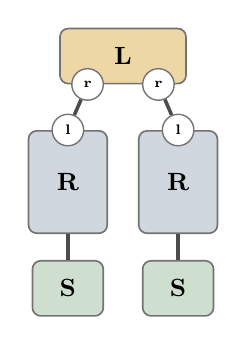
\begin{tikzpicture}[x=1cm,y=1cm]
  \node[molbox,fill=fsGold!40,minimum width=1.6cm] (L) at (0,1.6) {L};
  \node[site] (L1) at ($(L.south)+(-0.45,0)$) {r};
  \node[site] (L2) at ($(L.south)+(0.45,0)$) {r};
  \node[molbox,fill=fsNavy!20,minimum width=1cm,minimum height=1.3cm] (R1) at (-0.7,0) {R};
  \node[molbox,fill=fsNavy!20,minimum width=1cm,minimum height=1.3cm] (R2) at (0.7,0) {R};
  \node[site] (R1l) at (R1.north) {l};
  \node[site] (R2l) at (R2.north) {l};
  \draw[bond] (L1) -- (R1l); \draw[bond] (L2) -- (R2l);
  \node[molbox,fill=fsGreen!25,minimum width=0.9cm] (S1) at (-0.7,-1.35) {S};
  \node[molbox,fill=fsGreen!25,minimum width=0.9cm] (S2) at (0.7,-1.35) {S};
  \draw[bond] (R1.south) -- (S1.north); \draw[bond] (R2.south) -- (S2.north);
\end{tikzpicture}
\end{document}
